\chapter{COMPLETE FABRICATION}
\label{ch4}
This report summarizes complete fabrication process.

\section{WING}
\label{s:ch4_wing_fab}
This sections discusses about the wing section.

\begin{enumerate}
\item \textbf{Spar} : The spar is made of Aluminium rod of length 1.6 meters and having a cross-section of 1cm x 1cm
\item \textbf{Ribs} : Sixteen ribs are being used in the wing, each having thickness of 8mm and lenght 14.8cm, and have been made out of balsa wood. 
\item \textbf{Aileron} : The Ribs have been cut at 20\% from the trailing edge of the ribs. The control surface covers 60\% of the wing span.
\item \textbf{Hinges} : The Aileron section is attached to the main wing ribs using CA Hinges. All the Aileron sections are connected by a sheet of balsa wood which is then connected to a Servo which controls its motion.
\end{enumerate}

\section{FUSELAGE}
\label{s:ch4_fuselage_fab}
This sections discusses about the fuselage section.

\begin{enumerate}
\item \textbf{Frame} : As outlined in the previous chapter on Fuselage Design ( Chapter 4 ), the fuselage frame is a truss structure.
\item \textbf{Primary Load Structure} : Aluminium rod has been used to take the primary loads being transferred to the fuselage.
\end{enumerate}


\section{HORIZONTAL TAIL}
\label{s:ch4_horztail_fab}
This sections discusses about the Horizontal section.

\begin{enumerate}
\item \textbf{Spar} : The spar is made of Carbon Fiber rod of length 0.5 meters and has a cross-section of 2mm x 2mm
\item \textbf{Ribs} : Eight ribs are being used in the wing, each having thickness of 8mm and lenght 8.2cm, and have been made out of balsa wood. 
\item \textbf{Elevator} : The Ribs have been cut at 40\% from the trailing edge of the ribs. The control surface covers 90\% of the wing span.
\item \textbf{Hinges} : The Aileron section is attached to the main wing ribs using CA Hinges. All the Aileron sections are connected by a sheet of balsa wood which is then connected to a Servo which controls its motion.
\end{enumerate}

\section{VERTICAL TAIL}
\label{s:ch4_verttail_fab}
This sections discusses about the Horizontal section.

\begin{enumerate}
\item \textbf{Spar} : The spar is made of two Carbon Fiber rods. The main spar is a square Carbon fiber rod and is at an angle of $45\,^{\circ}$
 and has a cross-section of 2mm x 2mm. Additional vertical spar is being used to provide rigid support to the tail and is made of circular carbon fiber rod of length 16.2cm and cross-section having radius of 1.5mm 
\item \textbf{Ribs} : Six ribs are being used in the wing, each having thickness of 8mm, and have been made out of balsa wood. 
The Ribs have been cut at varying length by keeping the taper ratio in mind.
\item \textbf{Rudder} : The Ribs have been cut at 3cm from the trailing edge of the ribs. The control surface covers 90\% of the wing span.
\item \textbf{Hinges} : The Aileron section is attached to the main wing ribs using CA Hinges. All the Aileron sections are connected by a sheet of balsa wood which is then connected to a Servo which controls its motion.
\end{enumerate}

\begin{figure}[H]
    \begin{center}
      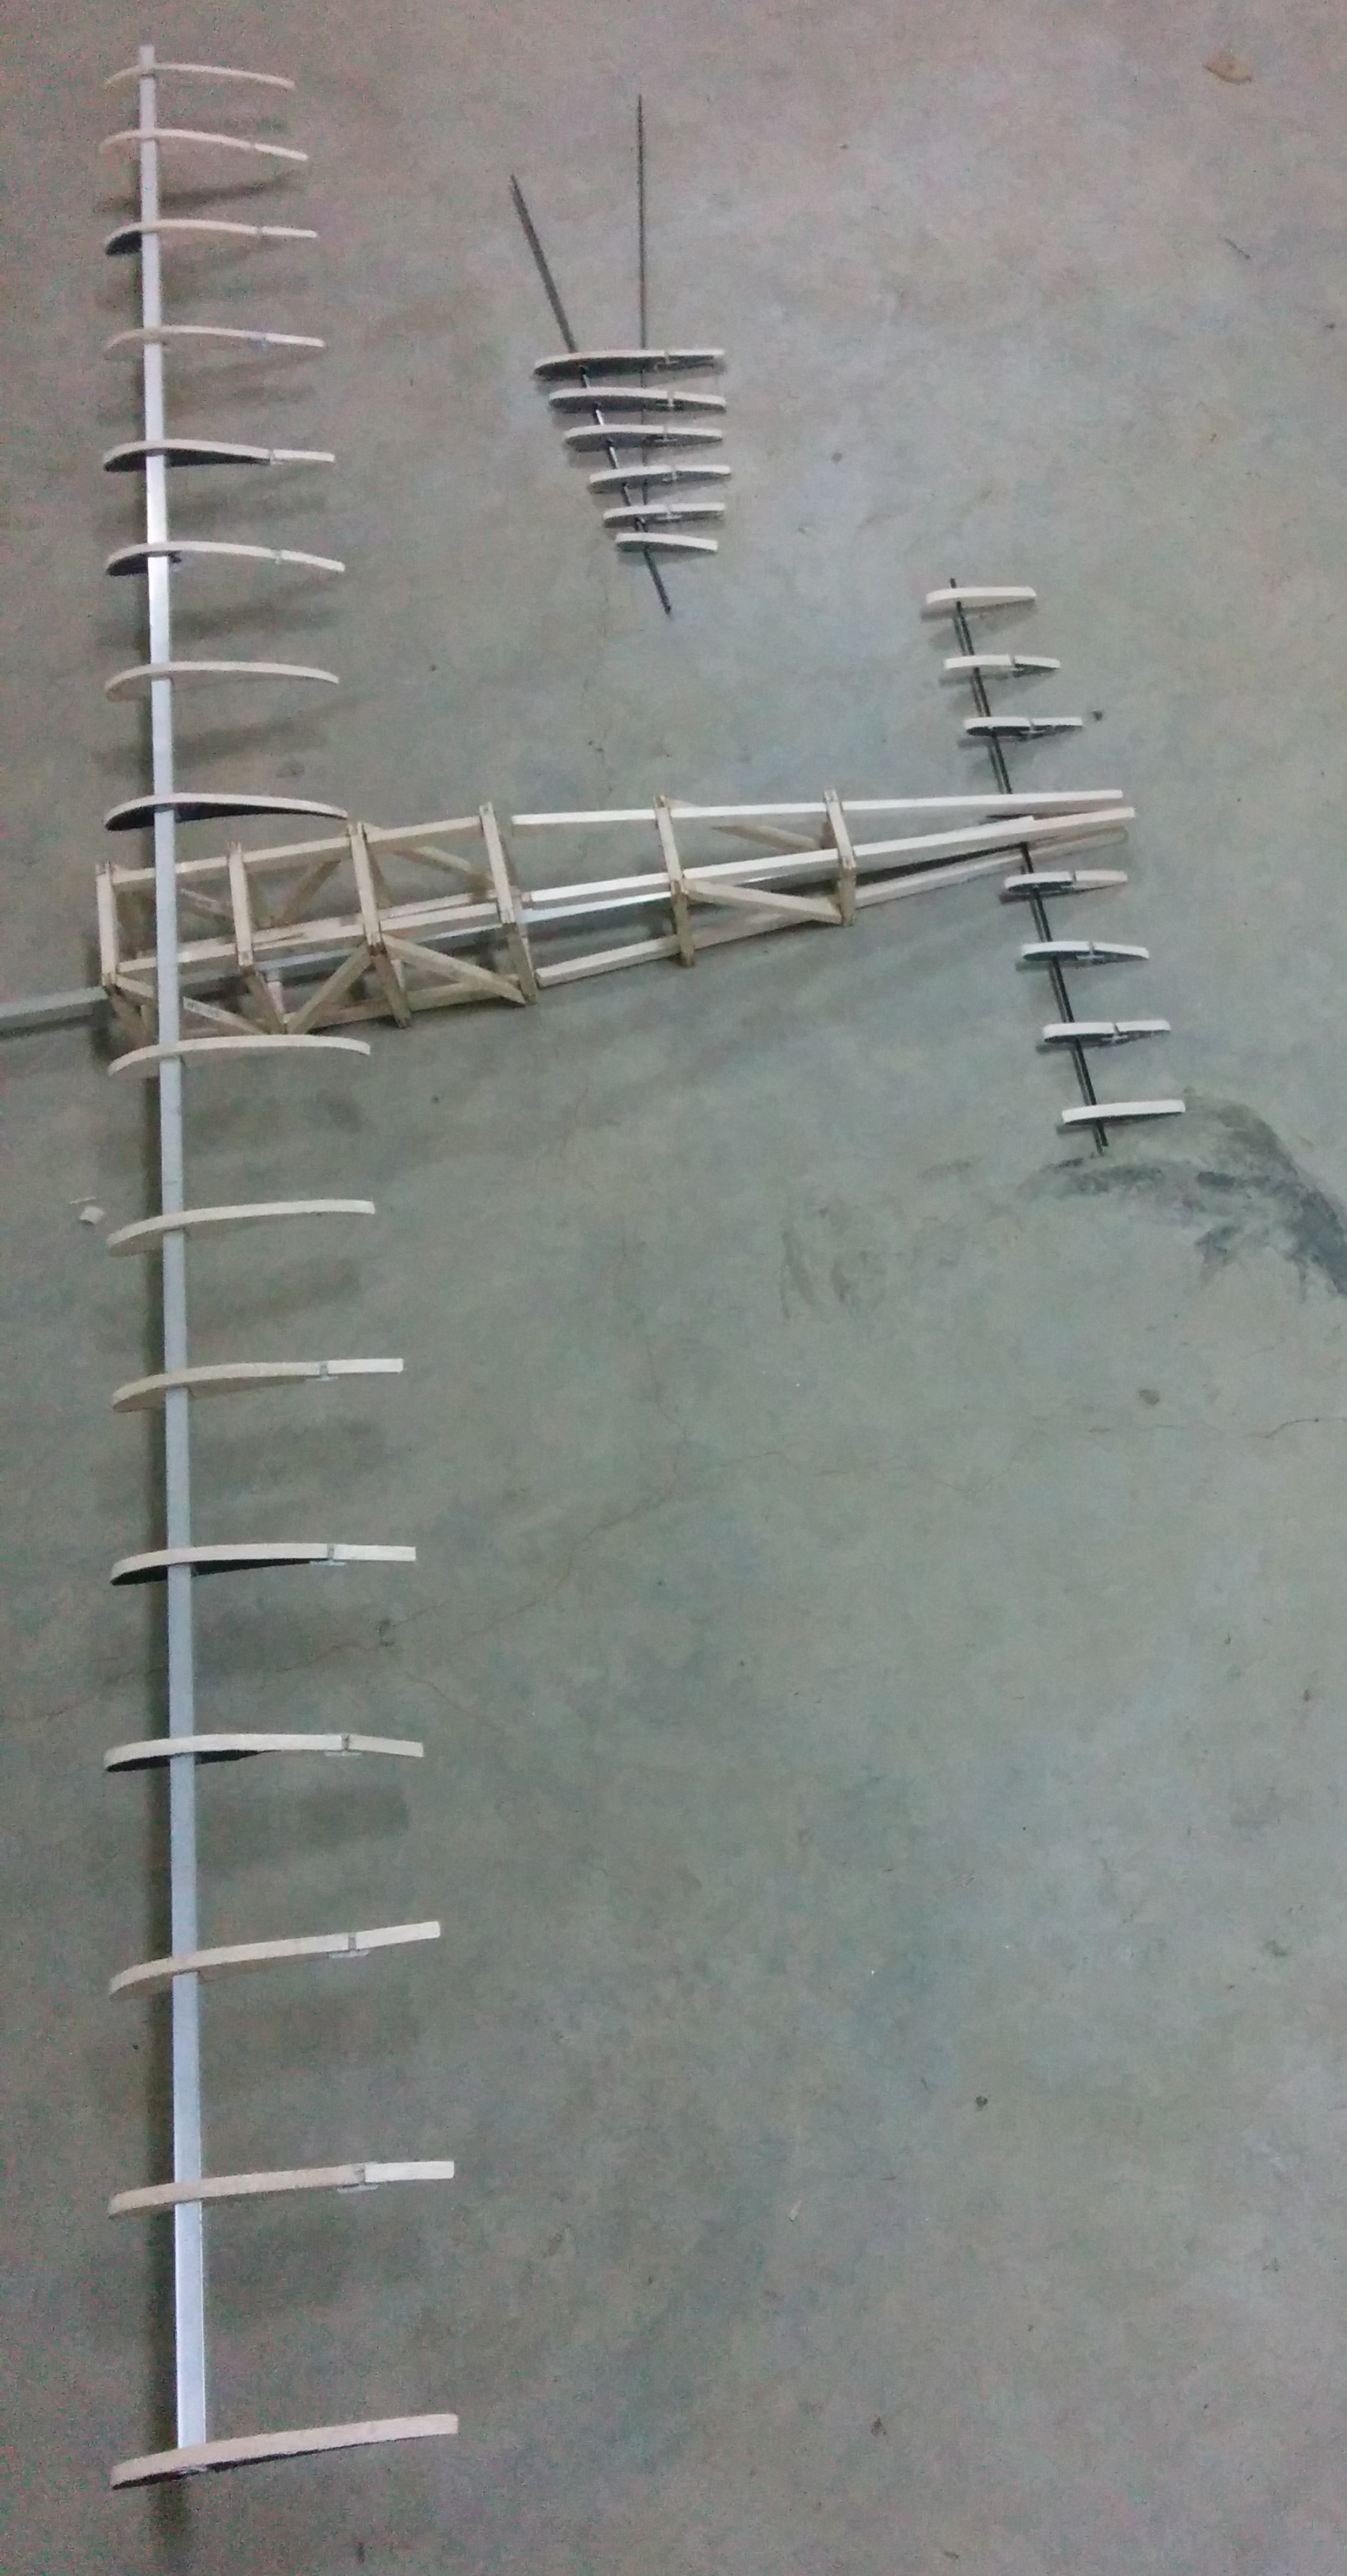
\includegraphics[width=5.1in]{figures/ch4_fab.jpg}
\caption{Complete Fabrication}
       \label{fig:ch4_fab}
    \end{center}
\end{figure}


%
